\section{Methods}
We constructed a deterministic compartmental \SVEIR
(susceptible, vaccinated, exposed, infectious, recovered)
model of \MPXV transmission.
The modelled population aimed to represent the Ontario \GBMSM community,
and included two levels of sexual risk (higher, lower)
and two weakly connected transmission networks (cities A, B).
Figure~\ref{fig:model.city.risk} illustrates the modelled city/risk strata,
Figure~\ref{fig:model.sveir} illustrates the \SVEIR health states, and
Table~\ref{tab:model.params} summarizes the default model parameters.
\par
\begin{figure}
  \begin{subfigure}[b]{0.49\linewidth}
    \centerline{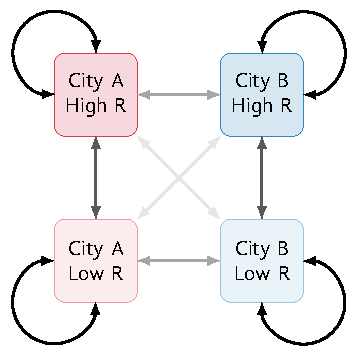
\includegraphics[scale=1]{model.city.risk}}
    \caption{Cities, risk groups, and contact networks}
    \label{fig:model.city.risk}
  \end{subfigure}\hfill
  \begin{subfigure}[b]{0.49\linewidth}
    \centerline{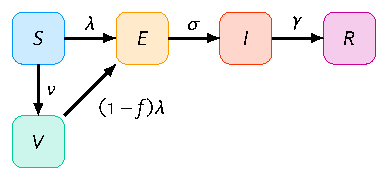
\includegraphics[scale=1]{model.sveir}}
    \vskip3em
    \caption{Health states and transitions}
    \label{fig:model.sveir}
  \end{subfigure}
  \caption{Model structure}
  \label{fig:model}
  \floatfoot
  (\subref{fig:model.city.risk})
  High/Low R: risk groups;
  arrow opacity is proportional to contact network connectivity between groups.
  (\subref{fig:model.sveir})
  $S$:~susceptible;
  $V$:~vaccinated;
  $E$:~exposed;
  $I$:~infectious;
  $R$:~recovered.
  See Table~\ref{tab:notation} and Appendix~\ref{app.model} for rate definitions.
\end{figure}
\begin{table}
  \centering
  \caption{Model parameters, including default values and ranges explored via grid sweep}
  \label{tab:model.params}
  \small
\begin{tabular}{llrcc}
  \toprule
  Parameter                          & Stratum                   &      Value &      Range       & Ref \\
  \midrule
  Population size                    & overall                   &    100,000 &                  & \cite{Wang2021}\tn{a} \\
                                     & fraction in city A        &        .50 &    [.20,~.80]    & \tn{a} \\
  Fraction higher risk               & city A                    &        .10 & [.01,~.50]\tn{b} & \cite{Wang2021}\tn{a} \\
                                     & city B                    &        .10 &                  & \cite{Wang2021}\tn{a} \\[1ex]
  Contact rate                       & close non-sexual, all     &          1 &                  & \tn{a} \\
                                     & sexual, low risk          &        .01 &                  & \cite{Wang2021}\tn{a} \\
                                     & sexual, high risk, city A & .178\tn{c} & [.10,~.25]\tn{b} & \cite{Wang2021,Endo2022}\tn{a} \\
                                     & sexual, high risk, city B & .178\tn{c} &                  & \cite{Wang2021,Endo2022}\tn{a} \\[1ex]
  Assortativity                      & cities, all contacts      &        .90 &    [.70,~1.0]    & \cite{Armstrong2020}\tn{a} \\
                                     & risk, close non-sexual    &          0 &                  & \tn{a} \\
                                     & risk, sexual              &        .50 &                  & \tn{a} \\
  Per-contact \SAR                   & close non-sexual          &        .05 &                  & \cite{Beer2019} \\
                                     & sexual                    &  .90\tn{c} &                  & \cite{Endo2022}\tn{a} \\[1ex]
  Initial infections                 & overall                   &         10 &                  & \tn{a} \\
                                     & fraction in city A        &        .50 &    [0.0,~1.0]    & \tn{a} \\[1ex]
  Duration of period                 & latent/incubation         &          7 &                  & \cite{Charniga2022,Thornhill2022,Miura2022} \\
                                     & infectious/symptoms       &         21 &                  & \cite{Adler2022,Thornhill2022} \\
  Fraction isolated among infected   &                           &        .50 &                  & \cite{Thornhill2022}\tn{a} \\[1ex]
  Vaccines available                 &                           &       5000 &                  & \tn{a} \\
  Vaccine effectiveness\tn{d}        &                           &        .85 &                  & \cite{Fine1988,PHAC2022vax,CDC2022vax} \\
  Vaccine prioritization sensitivity & high risk                 &        .90 &                  & \cite{TPH2022vax}\tn{a} \\
  Vaccine allocation                 & city A                    &        .50 & [0.0,~1.0]\tn{e} & --- \\
  \bottomrule
\end{tabular}
\floatfoot
All durations in days; all rates in per-day.
\SAR: secondary attack rate.
\tnt[a]{Assumed / representative.}
\tnt[b]{Calculated to fit $R_0 \in [1,2]$.}
\tnt[c]{Calculated to fit $R_0 = 1.5$,
  reflecting pre-vaccination estimate of \MPXV $R_0$ in Ontario \cite{PHO2022ont}
  via \cite{EpiNow2}.}
\tnt[d]{Leaky-type.}
\tnt[e]{Optimized parameter.}
\end{table}
\par
We initialized all model runs with 10 imported/seed cases,
distributed across the exposed and infectious stages proportionally by mean stage duration.
We then simulated distribution of 5000 vaccine doses over 15 days from day 60,
doses that were imperfectly prioritized to the higher risk group with 90\% sensitivity
--- i.e. 4500 doses reach the higher risk group and 500 each the low risk group.
\par
Using this model, we explored optimal vaccine allocation between cities A~and~B
over a range of epidemic conditions.
For a given set of conditions, we defined the optimal vaccine allocation as that which
resulted in the fewest cumulative infections by day 120 in both cities.
\par
We chose this 60-day time horizon and fixed 5000 vaccine doses to reflect
a plausible medium-term optimization problem relevant to the early \MPXV situation in Ontario.
In reality, multiple changing time horizons may require consideration,
different numbers of doses may become available, and
different rates of vaccination may be possible.
We aimed to obtain generalizable insights about the relationships between
specific epidemic conditions and efficient geographic prioritization of vaccines during an outbreak.
\par
As one specific example setting, we chose parameters representative of
Toronto (city~A) and another medium-sized Ontario city (city~B).
Based on 
\dots
80,000 and 20,000 \GBMSM population size, respectively.
\dots
10\% sexual network connectivity ($\epsilon_c = 0.9$).
\dots
$R_0$ = 2.0 in Toronto versus 1.5 in city~B.
\dots
100\% imported/seed cases in Toronto.
\dots
We then compared two strategies of vaccine allocation by city:
(a) proportional to population size; and
(b) fewest infections by day 120.%
\footnote{Optimal allocation was identified using the
  \href{https://www.rdocumentation.org/link/optimize?package=stats}{\texttt{optimize}} function in R.}
\par
Additionally we performed a ``grid sweep'' of the following epidemic conditions,
and identified the optimal vaccine allocation between cities A and B for each combination of conditions:
\begin{itemize}
  \item relative size of city A versus B (1/4~to~4 times)
  \item relative epidemic potential in city~A ($R_0$ in city~A from 1~to~2, versus fixed 1.5 in city~B),%
  \footnote{City-specific $R_0$ calculated assuming no inter-city mixing.}
        adjusted via the sexual activity of the higher risk group in the city~A
  \item between-city mixing (0~to~30\% of all contacts formed randomly between cities)
  \item fraction of imported/seed cases in city A versus B (0--100\%)
\end{itemize}


